% vim:linebreak:

\documentclass{report}
\usepackage{ohm-ngc}
\usepackage{url}
\usepackage{graphicx}
\usepackage{moreverb}
\usepackage{listings}

\lstdefinestyle{nonumbers}{language=C++,basicstyle=\small\ttfamily,frame=lines,captionpos=b,float=ht}
\lstdefinestyle{numbers}{language=C++,basicstyle=\small\ttfamily,numbers=left,numbersep=5pt,frame=lines,captionpos=b,float=ht}

\begin{document}

\title{System Support for Developing Recoverable Device Drivers}

\author{Hiroo Ishikawa, Alexandre Courbot and Tatsuo Nakajima}
{Waseda University\\3-4-1 Okubo, Shinjuku-ku Tokyo 169-8555 JAPAN}

\E-mail{\{ishikawa,alex,tatsuo\}@dcl.info.waseda.ac.jp}
\date{6 November 2008}

\begin{abstract}
System software, and device drivers in particular, are particularly prone to errors, with serious consequences for the system: failures in monolithic kernels usually corrupt the whole system. This situation is particularly a problem in embedded systems where maintenance is not possible. Microkernels increased the robustness to such failures by compartmentalizing system components, but do not take their recovery into account, often leading other system components and applications that depend on the failed component to fail in turn.

In this paper, we address the problem of system components recovery in microkernel-based operating systems. In order to increase the chance of successful and transparent recovery, we propose a device driver development framework that takes recovery into account and let the driver developer specify the meaningful state of the driver, as well as the recovery policy. Giving such control to the device driver developer allows us to significantly improve recovery of failed drivers, by erasing and reconstructing meaningless driver state and reprocessing the failed request in order to keep the failure transparent to the rest of the system.
\end{abstract}

\begin{keywords}
% about 5 words
device drivers, resiliency, self-recovery, persistent memory
\end{keywords}

% Improve the evaluation
% Clarify the relation to the Crash-only software
% Give guidelines/principles of driver construction
% How to handle the complexity due to the recovery code
% Cite the SASO08 paper

\section{Introduction}

Resiliency of embedded software systems is necessary in order to compensate their lack of administration means.  The more complex software systems in mobile devices and car electronics become, the more complicated their maintenance becomes.  Since users are usually not specialists in computer systems, such embedded systems are required to recover themselves from runtime failures.  Rich administration means do not solve this problem because the knowledge of computer systems is more or less required to use them, knowledge which we cannot expect end users to have.  It is thus crucial for these systems to have recoverability that keeps the soundness of system state.

% Mention about transparency

Although recoverability is required for any layer of a system, our research focuses on the operating system layer.  An operating system is usually implemented in a low-level programming languages such as C and assembly, which requires programmers to give a lot of attention to their programs.  Moreover, failure in an operating system is critical to continue operations of the entire system.  We are particularly interested in device drivers because they are prone to errors:  some research indicates that device drivers includes more bugs than the other kernel code\cite{Chou2001}.  Additionally, failure of device drivers is likely to crash the whole system.

Prior research adopts restarting as the main method of failure recovery of device drivers\cite{Swift2006}\cite{Herder2007}, and our research follows this method.  Restart recovery isolates a device driver from other operating system components so that it can be restarted while the other services continue their processing.  The prior approaches allow device drivers to be developed in such a way that developers do not have to think about their failure recovery.  Hence, only stateless device drivers can be safely recovered by restarting, or a system is required to involve a heavy-weight recovery mechanism such as checkpointing.  In general, checkpointing is insufficient for the embedded systems and device driver recovery in terms of memory consumption and hardware state management.  Although our approach requires partial information of device drivers through a template for writing a device driver, the recovery mechanism is light-weight and recovery is efficient.

We proposed a framework for writing self-recoverable device drivers\cite{ishikawa08a-framework}.  By cooperating with driver developers, we achieved to transparently recover not only stateless device drivers but also drivers with an internal state.  This paper describes about the framework in detail.  Under the framework, a failed driver is simply restarted by a privileged program inside the operating system.  A driver with internal state is required to synchronize its state with managed peripheral and/or clients.  To manage driver's internal state, our framework provides a light-weight persistent memory that preserves important state across restart.  The driver framework also provides a template to write a device driver.  A driver developer can write a recoverable device driver by following the template.  The light-weight persistent memory is easy to use and involves no access overhead.  The framework is developed on top of L4 microkernel\cite{L4X2} which is commonly used solution in contemporary embedded systems.  Hence, device drivers run in user mode and are isolated from each other to limit the propagation of failures inside the operating system.

To evaluate the feasibility of our framework, we conducted several case studies, and a fault injection test for each case.  We implemented a parallel port, a video card, and an audio drivers, which the previous approaches were unable to recover efficiently, because all these device drivers involve internal state to be preserved across restart.  In particular, we inject a fault into an audio device driver where a recovery process is required not to create a gap in its output.  Unlike a character device driver that our previous work addressed, an audio device driver has a harder requirement for downtime due to recovery.

The reminder of this paper is structured as follows:  Section 2 and 3 describes the design and implementation of our framework.  Section 4 shows several basic evaluation and conducts a series of case studies on the framework.  Section 5 discusses the current limitations and further issues of the framework.  Section 6 concludes the paper.


\section{A Framework For Recoverable Device Drivers}
\label{s:design}

In this section, we describe the design of our framework for recoverable device drivers. It provides a simple way to write drivers that is consistent with the programming model of L4, and also gives the tools necessary for the programmer to consider recovery. Its recovery procedure is to restart the failed driver while preserving data that the programmer has marked as significant for the driver's consistency and transparent recovery.

\subsection{Failure Model}

Lowell et al. \cite{Lowell2000} made a classification of software failures. They distinguish between \emph{stop failures} (i.e. a program stopped because of an external reason, such as a \emph{kill} signal or a power outage) and \emph{propagation failures} (the program stopped because of an internal bug that drove it into a unacceptable state). Stop failures are easy to recover, as the interruption cause is external to the program. Therefore, provided an earlier snapshot of the running program is available, it is usually enough to restore it and pursue the execution of the program, that will this time pass the failure time successfully if the external factor that stopped it previously is not repeated again.

More challenging are propagation failures. These failures are caused by a transient bug\footnote{A transient bug or Heisen-bug is a bug that only appears occasionally and is not easily repeatable\cite{Gray1985}.} into the running program. The time of failure and time of bug usually differ --- and can be very distant. Moreover, figuring out when the bug entered the program at the time of failure is extremely difficult. As a consequence, restoring the program to a previous state does not ensure recovery, as it is very possible that the restored state is already contaminated by the bug and will identically lead to a failure. Moreover, even if the system is restored to a state prior to the bug, nothing can ensure that the buggy conditions will not appear again during the next run.

The framework tries to recover crash and fail stop failures.  A crash is a failure that violates the requirements of the underlying system.  A driver crashes because it violates the specification of the CPU, the MMU, or a peripheral, for instance, by dividing a number by zero or accessing a prohibited memory area.  Stop failures make a component unresponsive to a communication.  This type of failure can be detected through the kernel or a report from a component that interacts with the failed component.

The framework is designed to handle transient failures.  Transient failures are caused by a panic due to an inconsistency of the component internal state, race conditions, software aging, particularly memory leaks.  Our basic approach to transient failures is to restart a failed component so that the failure disappears with the next run.

% Limitations
Since the framework focuses on transient failures, which occur non-deterministically, deterministic failures are not currently supported.  Previously, we mentioned that transient failures are caused by a panic, but another panic such that is caused by a message to the component, ends up with a permanent failure.  In this case, it is necessary to repair the contents of the message.  Restarting the source of the message is likely to recover such failures.



\subsection{State of Drivers Across Recovery}
\label{s:fw}

As described above, the main issue with transient propagation failures is that they corrupt the state of the program, and invariably lead to a failure unless the corruption is cleared. Therefore, clearing the state of the failed program (e.g. through a complete restart) is the most efficient way to recover the software.  However, this extreme solution is not acceptable for all device drivers because the internal state of the driver is then completely lost.

{\it Crash-only software}\cite{candea03crash-only} also encourages to separate data relevant to the internal state of a software component from its control.  While the application of crash-only software is Internet applications, our focus is device drivers.  Internet applications assume databases store their significant data, and the database maintains data consistency even across failure.

Our strategy for recovery is to clear as much of the driver's state as possible, while preserving its essential state. We restart the driver completely, but preserve certain data that the programmer marked as significant for recovery.  Upon restart, the driver is branched to an alternate entry point that is responsible for restoring its state from this persistent data. Once recovery is over, the driver can reprocess the request that caused its failure. Upon this restart, we expect that the reprocess will not generate the same error.

There are two design issues that derive from this statement:
\begin{enumerate}
\item Upon driver restart, the failing operation must be performed again.
\item The framework must be able to preserve data that is significant to the state of a driver and its managed hardware. This generally includes any data that cannot be recomputed identically to the pre-failure condition.
\end{enumerate}

The first requirement is easily satisfied by the design of microkernels.  In microkernels, device drivers, like any other system part, are user-space servers that reply to requests arriving in the form of messages. By including this design into our framework, it is easy to consider message processing as the atomicity of our recovery system, and to reprocess the message that triggered the failure once the driver is recovered.

As for the last requirement, the difficulty of discriminating between significant and insignificant data is what makes recovery of propagation errors difficult. If not enough state is dropped, the corruption of the system state may survive the recovery; on the other hand, if too much state is reinitialized, complete recovery is not possible and the behavior of the recovered driver may differ from its normal operation. As a recovery framework cannot decide what differentiates useful from futile state, we decide to let the programmer directly specify which of its variables should survive a recovery. In general however, the following rules are applied.

\paragraph{Significant state}
The state that should be preserved is classified into the following categories.
\begin{itemize}
\item Driver data that reflects the state of the hardware.  If a driver and its managed hardware are out of sync, there is a high chance that the next commands issued by the driver will put the hardware into an inconsistent state.
\item Internal driver state that must survive across requests. This may include state that deals with data being provided by the managed hardware. For instance, if a character device driver sends data to the hardware from a buffer at the time of failure, recovery must be aware of the position at the time of failure in order to avoid sending the same data again.
\end{itemize}

\paragraph{Non-significant state}
State that is local to the processing of a request and is not significant as long as a side-effect that depends on it has not been performed by the driver. All the input data of a request is contained into the incoming message, that is replayed once the driver is restarted. Therefore, it is safe and desirable to discard any local data created during this process, as it is likely that the corruption occurred there. Our policy of restarting the driver (even though through an alternate entry point) ensures that all local state is discarded.

%The significant state is classified into the following two types of data according to their scopes.
%\begin{description}
%\item[Global scope (significant state)]
%Data in the global scope is data shared by all the procedures of a device driver.  The global data is separated two more types.  Soft-global is the global data of software, such as a container object for saving client information.  Hard-global is the data and configurations on managed hardware, such as video mode information of VESA and the buffer on a NIC.
%\item[Session scope (significant state)]
%Data in the session scope is referred to data that should preserved across requests.  It is mainly the information related to clients, including pages shared with clients and resource handlers held by clients.  For instance, a file descriptor is a kind of the session data.
%\end{description}

%The non-significant state is also classified into two types.
%\begin{description}
%\item[Request scope]
%Data in the request scope is data that is available while a handler processes a request.
%\item[Local scope]
%Data in the function scope is data that is local to a handler such as local variables in a function.
%\end{description}

%Data in the global and the session scopes may be shared among handlers, but the rest is not (as far as we assume that one request is handled by one handler).  Obviously, the significant state is the global or the session scope.


\subsection{Architecture of ArcOS}
\label{s:arc}

ArcOS is a multiserver operating system built on top of the L4 microkernel~\cite{L4X2} (Fig.~\ref{fig:arc}).  L4 provides minimum fundamental abstractions such as threads, IPC (for \emph{inter-process communication}), and address spaces. System components such as drivers run in user mode and are isolated by protection domains that are crucial for fault containment. ArcOS currently runs on the Intel IA32 architecture.

\begin{figure}[ht]
\centering
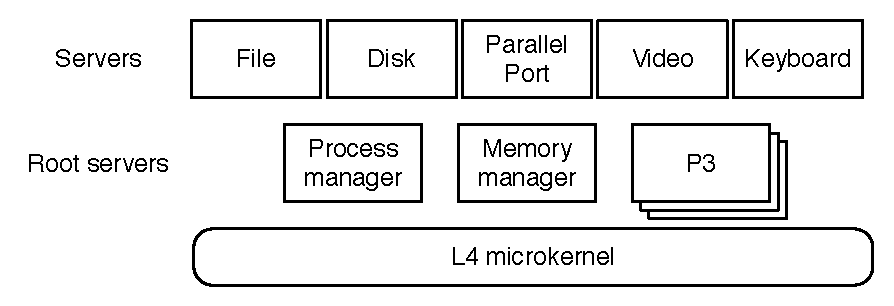
\includegraphics[scale=0.6]{architecture}
\caption{Architecture of ArcOS}
\label{fig:arc}
\end{figure}

A process under ArcOS communicates with other processes via the L4 synchronous IPC mechanism. Since an IPC message payload is limited to tens of bytes, processes can use shared memory pages to exchange large amounts of data. The IPC state of a process, as well as memory page faults, are handled by its pager, a dedicated process called P3 (for \emph{Per-Process Pager}, see Fig.~\ref{fig:p3}). The pager is also in charge for loading the program, which confers it a crucial role in recovery.

\begin{figure}[ht]
\centering
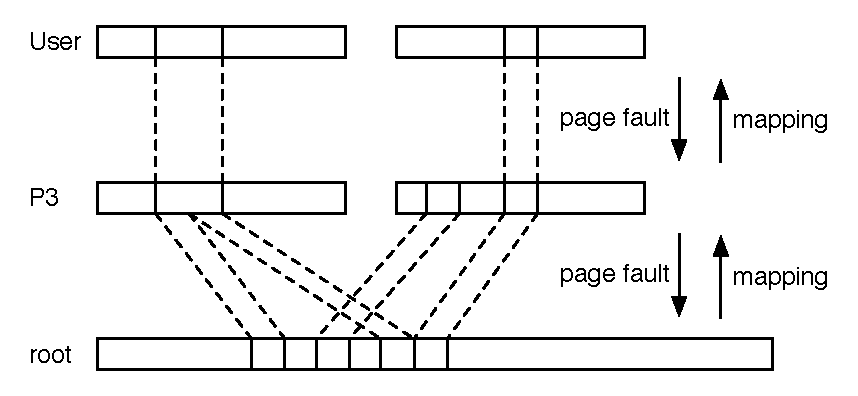
\includegraphics[scale=0.6]{p3}
\caption{The root pager, per-process pagers and user processes}
\label{fig:p3}
\end{figure}

This particular design, in which P3 acts as a ``nurse'' for the process it manages, increases the isolation of processes and influences how our recovery mechanism will perform.

All server processes under ArcOS including device drivers follow the single-threaded event-handler architecture.  The event handler architecture is much simpler than multithreaded architecture\cite{ousterhout96why-threads} and thus more reliable.  Multithreading is not necessary for a device driver which uses only one thread to control the hardware.

\subsection{Design of the Framework}
\label{sec:design-framework}
Just like any other process, a device driver is loaded and started by its own instance of P3. This particularity greatly influences the design of our driver framework. First, the task of putting the driver back into recoverable operation is left to P3. Also, the driver can have different entry points, depending on whether it is being recovered or not. We consider that there are four main states in the life of a device driver:

\begin{description}
\item[Initialization.]
Where the device driver initializes the managed hardware and its internal data structures. This state is only entered once, when the driver is initially started.

\item[Service loop.]
In ArcOS, a device driver is a server process, which waits for requests from its clients: for instance, a file system server is a client of a disk driver. The service loop implements that request handling mechanism, by associating messages to handler methods.

\item[Finalization.]
In case of normal termination of the driver, it may be necessary to prepare to exit by synchronizing the hardware state to the current driver state, or safely terminating the current sessions with its clients.

\item[Recovery.]
Every device driver is supposed to implement its crash recovery procedure. Should a failure occur within the driver, the framework restarts it and invokes this function instead of the initialization function. It is then up to the recovery function to ensure the driver is put back into a state where it can work again safely, by using the recovery mechanisms provided by the framework.
\end{description}

When the driver is initially started, the initialization function is called by P3, followed by the service loop and the finalization function. Should a failure occur while the driver is processing a service request, the non-persistent part of its address space is reinitialized and the driver is reloaded, entering this time the recovery function before pursuing on the service loop again (Fig.~\ref{fig:driverstatemachine}).

\begin{figure}[ht]
\centering
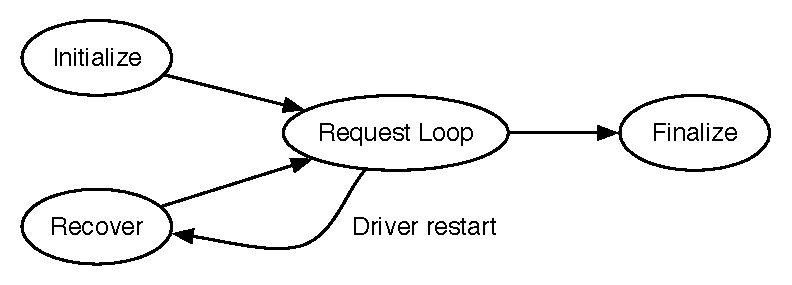
\includegraphics[scale=0.6]{driverstatemachine}
\caption{States of a device driver.}
\label{fig:driverstatemachine}
\end{figure}

The framework is designed as a wrapper around the actual driver that provides this basic shape as well as other facilities for recovery (Fig.~\ref{fig:fw}). Using it, the driver writer only has to write behaviors for the initialization, finalization and recovery functions, define the protocol used by the driver to communicate with client processes, and associate function handlers to the different kinds of messages the driver can handle. Both message and error handling are then performed by the framework on this basis.

\begin{figure}[ht]
\centering
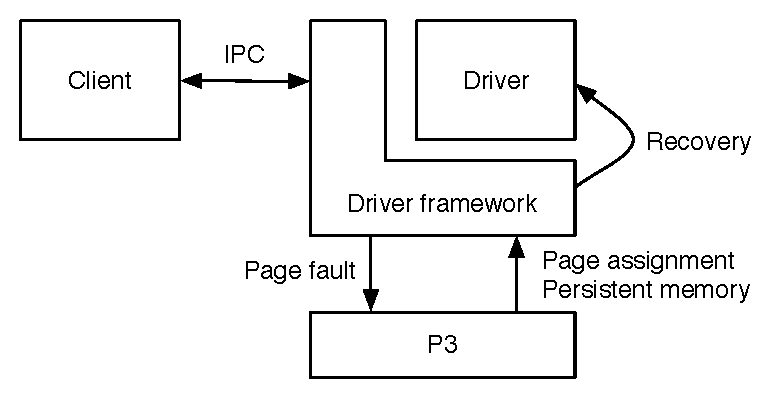
\includegraphics[scale=0.6]{framework}
\caption{Device driver framework}
\label{fig:fw}
\end{figure}

Memory management and failure detection are performed by P3 which, as the driver's pager, is immediately notified of page faults and other error conditions. Should P3 detect an invalid behavior of the driver (such as a page fault to an unauthorized address, or a division by zero), it will immediately stop the driver and restart it from the recovery entry point. During the driver restart process, all its address space is cleaned and reset to its initial state, with the exception of the persistent memory area which is the only state of the driver that survives failures.

\subsubsection{Persistent memory}

When the driver fails and is restarted by P3, it tries to recover to a state that is consistent with the state of the hardware being managed so that the crash and recovery are completely transparent to other processes. Restoring to the pre-crash state requires that the data relevant to this state survives the crash. To this end, the framework provides a persistent memory area for every driver.  This area is mapped to a specific region in the driver's address space that holds data across process restart - but does not survive normal termination of the program.  Unlike a file system, the data in the persistent memory area is mapped to the physical memory so that a program deals with it as for with non-persistent data.

The framework provides a specific keyword that can be appended to variable declarations in the source code and results in these variables ending into the persistent memory area. Such declared variables remain untouched by the recovery process, and remain accessible via their pre-crash address as soon as the driver is restarted.

It is the responsibility of the driver writer to mark data that is relevant to recovery as persistent. On the other hand, the set of persistent data should be as small as possible to reduce the risk of contaminating the persistent area with a propagation fault, which would result in the same failure to occur after recovery. To this end, the policy that we used during our own drivers development is to first write the driver without recovery in mind, and then make the slight adaptations that are needed to use our recovery framework. That way, variables that end in persistent memory are well-thought and chosen accordingly to the final design of the driver. We will discuss this point furthermore in the implementation and experiments sections.


%\subsubsection{IPC continuation and disruption}
% Assuming single-threaded
%As every communicating process does, a device driver maintains its own IPC state.  Under our framework, in which the driver is a server replying to client requests, the state of IPC is always preserved across restart.  However, if the driver crashed before replying to the client (which is what happens unless the bug resides within the framework itself), leaving IPC state may block the client that is waiting for the reply from the driver.  To solve this problem, the framework always stores the last message it received in the persistent memory area.  In case of recovery, the last message can therefore be reprocessed. Consequently, outside processes do not notice any interruption of service.

%It shall be noted that a failed request may be processed differently in case of recovery. Requests that ask a character device driver to write or read more than one unit of data from the device may rely on a buffer and an iterator. In this case, replaying the whole request from start would result in data being written multiple times or previously read data being erased. Therefore, the handler function must be aware that the handled request is a replay of a failed previous one to behave properly. This is  possible thanks to a global status variable that is set by the framework before processing a failed request.


\subsubsection{Recovery policy}

Our recovery method is based on restart recovery.  If a driver fails, the framework restarts it to remove the cause of the failure.  The framework first tries to preserve the persistent memory when restarting the driver.  If the same failure occurs despite of recovery, the framework then performs a full restart of the faulty driver.

\section{Implementation}
\label{s:impl}

ArcOS is implemented on top of L4::Pistachio\cite{L4X2} with experimental features. In accordance to ArcOS philosophy, both the framework and device drivers are implemented in C++.  By means of inheritance, the framework enforces device drivers to implement the recovery operations.  The framework runtime implements common operations such as the server main loop and the definition of recovery operation flow, as well as the persistent memory.

\subsection{Driver Framework}

The framework provides the \texttt{DeviceDriver} base class that enforces that all device drivers provide the mandatory operations we described in Section~\ref{sec:design-framework}. Listing~\ref{fig:devicedriverclass} shows a simplified version of the declaration of this class.

\begin{lstlisting}[style=nonumbers,caption=Simplified version of the DeviceDriver class declaration.,label=fig:devicedriverclass]
class DeviceDriver {
protected:
  virtual status_t Service(const L4_ThreadId_t& tid,
                           const L4_Msg_t& msg,
                           L4_Msg_t& retMsg) = 0;
public:
  virtual status_t Initialize() = 0;
  virtual status_t Exit() = 0;
  virtual status_t Recover();
  status_t MainLoop();
};
\end{lstlisting}

The \texttt{Initialize} and \texttt{Exit} methods are pure virtual, which enforces the driver developer to implement them. \texttt{Recover} is virtual but the framework provides a default implementation that just returns an error message to P3, stating that the driver cannot be recovered and causing a full-restart of the failed driver. Therefore, it is possible and easy to write device drivers without taking the recovery aspect into account.

The other public function, \texttt{MainLoop}, is already implemented and is called by P3 after the driver is started or recovered by \texttt{Initialize} or \texttt{Recover}. It waits for incoming messages, and passes them to the \texttt{Service} method along with the identifier of the sender. It also replays the failed request in case of driver recovery.

The \texttt{Service} method, although declared as pure virtual, is not to be implemented directly by the driver's writer, contrary to the other methods. This method mainly consist of a \texttt{switch} statement that checks the label of the incoming message, calls the corresponding handler, and puts the message to return to the client into \texttt{retMsg}. As it must deal with error handling and is very repetitive, we wrote a set of macros that construct that method using the message/handler paradigm to associate message labels to the corresponding method handler. An example usage of these methods is given by Listing~\ref{fig:connectors}.

\begin{lstlisting}[style=nonumbers,caption=Example usage of the message/handler macros.,label=fig:connectors]
BEGIN_HANDLERS(AudioDriver)
CONNECT_HANDLER(AUDIO_SET_VOL, SetVolume)
CONNECT_HANDLER(AUDIO_FLUSH_BUF, Flush)
...
END_HANDLERS
\end{lstlisting}

The message labels (e.g. \texttt{AUDIO\_SET\_VOL}, \texttt{AUDIO\_FLUSH\_BUF}) are just integers that define the protocol used between the client and the driver and may be build using an enumeration. Handler functions such as \texttt{SetVolume} and \texttt{Flush} must follow the following prototype:

\begin{lstlisting}[style=nonumbers,caption=Handler function prototype.,label=fig:handler]
status_t HandlerFunction(const L4_Msg_t& msg,
                         L4_Msg_t& retMsg);
\end{lstlisting}

They return the message that is to be sent back to the client in \texttt{retMsg}.

This framework provides all the building blocks to write a device driver for ArcOS. By just being required to write the initialization and finalization methods and to connect messages to their corresponding handlers, the driver writer can concentrate on the functional aspect of the driver without having to worry about inter-process communication. Once the driver is written, he can then take care of the recovery aspect.

Making a driver recoverable requires to write the corresponding recovery method, and to mark relevant data to be persistent across failures.

\subsection{Persistent Memory}

The persistent memory area is designed to host data that is necessary to recover and must survive a failure. Contrary to what can be expected from a persistent memory, it does not rely on external storage and simply consists of a special part of the main memory\footnote{Real persistent storage is not necessary here as the memory must only survive driver failures, not system restart.}. Its features make it particularly suitable for embedded devices:
\begin{itemize}
\item Very lightweight: no special management is required for persistent data, which is accessed like any other data in the main memory.
\item No data redundancy: persistent data is not a duplicate of existing data, but the actual runtime data mapped to a dedicated range of the address space.
\item Easy to use: a single macro to append to a variable declaration makes it persistent.
\end{itemize}

Implementation of this persistent memory is done through a cooperation of the compiler and linker. The GCC compiler\cite{GCCManual} provides support for section attributes that define the section of an ELF\cite{ELFSpec} file in which a declared variable should be located. By using this feature, we defined a C macro that can be appended to any declared variable in order to place it into a special \emph{.pdata} section.

\begin{verbatim}
#define IS_PERSISTENT __attribute__ ((section(".pdata")))
\end{verbatim}

At link time, the LD linker is given a special link script that relocates all data in the \emph{.pdata} section together. When P3 loads the device driver binary, it detects this \emph{.pdata} section and automatically maps it into a dedicated area of the address space (Fig.~\ref{fig:layout}).

\begin{figure}[ht]
\begin{center}
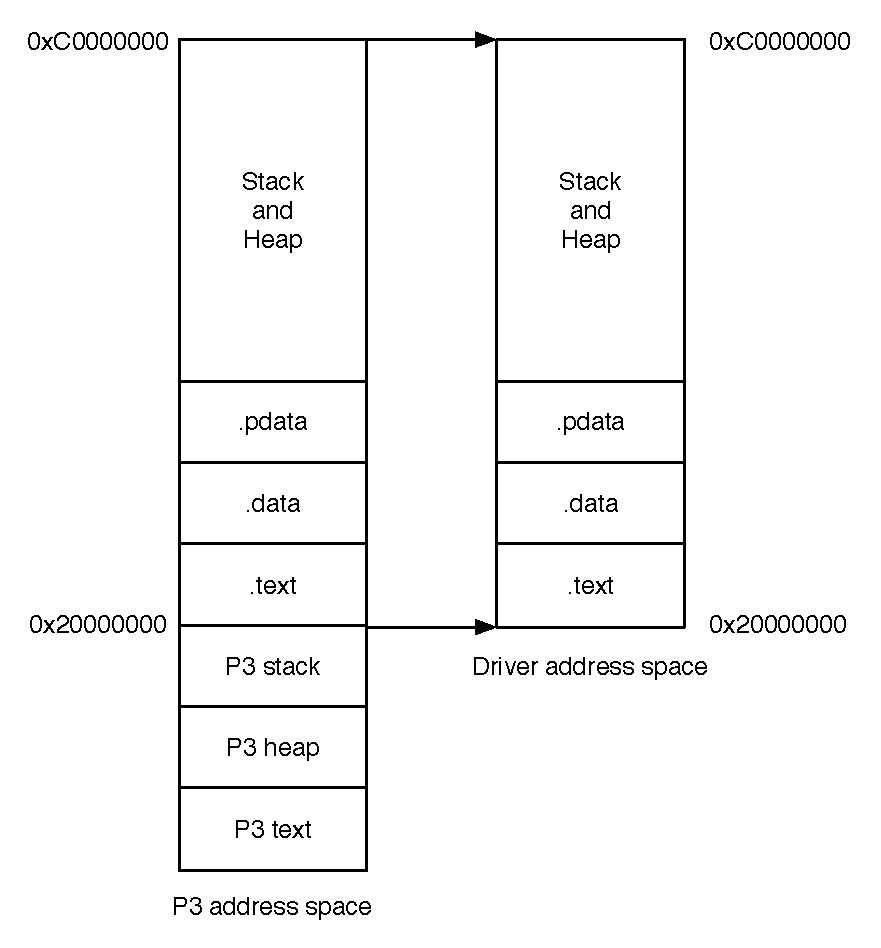
\includegraphics[scale=0.6]{layout}
\caption{The memory layout of a device driver process}
\label{fig:layout}
\end{center}
\end{figure}

Each process therefore has its own persistent memory area. P3 assigns physical memory pages to the persistent memory area at load time, just as it does with other memory sections. However, upon a failure of the driver process, all the physical pages but the persistent memory area are unmapped. This design makes the persistent memory area absolutely free in terms of memory footprint, and virtually free in terms of performance, since only a few trivial operations must be performed by P3 at load and recovery time to support it.

The Rio file cache uses a similar approach to provide persistent memory to applications\cite{chen96the-rio-file}.  While our implementation of persistent memory is allocated at compile time, Rio allows applications to allocate it at runtime.  This flexibility is an advantage of Rio to ours, however, applications need to salvage the Rio file cache upon a crash.  Since we aim to recover a crashed device driver in a short time to improve the system availability, we took the approach of using C macros.

We should note that this memory is not transactional. It is not possible to bring it back to a previous state: this means that if the failure propagates into the persistent memory area, it will most likely not be recoverable.

\subsection{Failure Detection and Recovery}
Error detection is performed by the P3 instance of the device driver, because it is in charge of handling page faults and other kinds of exceptions. Currently we only detect memory access violations.  However, it is possible to detect other types of failures such as fail-stop failure by cooperating with servers that interact with drivers, because a driver that suffers from a fail-stop failure doesn't respond.  It is possible to improve this mechanism to a general error detection architecture as proposed by Qin et al.\cite{Qin2007} or Wang et al\cite{Wang2006}.

The recovery process when an invalid page access (most likely due to an invalid pointer being used) occurs is as follows: first, the faulty driver is stopped, and all its memory pages but the code and persistent data sections are unmapped. Then, the data and heap area are recreated as for when the driver is initially loaded, and an initial stack is allocated. P3 then invokes the \texttt{Recover} method of the driver instance, which returns a status value: if that value indicates that recovery failed, P3 then fully restarts the driver from scratch. On the other hand, if the return value indicates a success, P3 sets the global recovery flag to \emph{true} and starts the driver by invoking the \texttt{MainLoop} method in the driver's address space.

The implementation of the \texttt{MainLoop} method first checks the value of the global recovery flag. If this value is \emph{true}, it immediately calls the \texttt{Service} method with the last message it received before the crash. Indeed, the received message and ID of the sender are themselves placed in persistent memory. Listing~\ref{fig:mainloop} gives a shortened version of the \emph{MainLoop} implementation, where the error handling code has been removed.

\begin{lstlisting}[style=nonumbers,caption=Shortened version of \texttt{MainLoop}.,label=fig:mainloop]
static L4_ThreadId_t tid IS_PERSISTENT;
static L4_Msg_t msg IS_PERSISTENT;

status_t DeviceDriver::MainLoop() {
  status_t err;
  L4_Msg_t retMsg;
  L4_MsgTag_t tag;
  if (Recovered) goto restore;
begin:
  tag = L4_Wait(&tid);
  for (;;) {
    ...
    L4_Store(tag, &msg);
restore:
    err = Service(tid, msg, retMsg);
    ...
    L4_Load(&msg);
    tag = L4_ReplyWait(tid, &tid);
    Recovered = false;
  }
  ...
\end{lstlisting}


\section{Evaluation}
\label{s:eval}

In this section, we would like to evaluate the efficiency of our driver framework. The main point for a recovery mechanism is to effectively recover upon failures. Therefore, we will first illustrate how we managed to recover on three different drivers instances: first, on a character device driver (parallel port driver), a class of devices that are reputed particularly difficult to recover because of the stream nature of the managed hardware. Then, we will consider recovering a VESA video driver. This kind of driver must keep enough information about the current state of the managed hardware to ensure a complete and transparent recovery (i.e. without graphical glitches or noticeable delay in display).  Finally, we will consider recovering a sound blaster audio driver which uses DMA and interrupts.

All our evaluations have been performed on an Intel Pentium4 3.4GHz with 1GB of main memory.

\subsection{Performance Evaluation}
\label{sec:performance}
We started by evaluating the overhead of P3.  P3 redirects all page mapping requests to the root pager, which holds the physical memory pages.  We measured the cycle count of handling a page fault and the subsequent page mapping.  Page fault handling with P3 takes approximately 1.5 times as many cycles as the one without P3.  Since page faults only occur the first time a user process accesses the page, we consider the resulting overhead as not critically harmful to performances.

Total downtime of the framework upon a failure has been measured to 0.2 ms.  To get this metric, we injected a simple fault that results in a memory access violation, and measured the time from the fault being triggered to the {\tt Recover} method being called.  Table~\ref{tbl:recovery} shows the detail of the downtime.  The {\it Unmap} operation unmaps all the pages mapped to the driver process excepted for pages of the persistent memory.  {\it Initialize} re-initializes the counterpart of the process inside P3, which manages the base address and the size of each segment.  {\it Load} reads the binary and extracts it to the main memory. {\it Start} triggers the driver process, however, the driver doesn't immediately run because none of its pages are currently mapped.  P3 thus invokes the IPC handler which deals with page mapping requests.  According to the table, program loading takes almost half of the total time, and the remaining time is consumed by page fault handling after the driver process is restarted.

\begin{table}[ht]
\centering
\caption{Measured recovery time}
\label{tbl:recovery}
\begin{tabular}{|l|r|r|} \hline
{\bf Operation}&{\bf Time}&{\bf Rate}\\ \hline
Unmap & 28.63us & 14.33\% \\ \hline
Initialize & 0.22us & 0.11\% \\ \hline
Load & 88.46us & 44.27\% \\ \hline
Start &  8.89us & 4.45\% \\ \hline
Mapping & 73.8us & 36.9\%\\ \hline
\end{tabular}
\end{table}

To these 0.2 ms of recovery time, must be added the time necessary to invoke the \texttt{Recover} method of the driver. The execution time of this method is obviously driver-dependent. For the drivers we evaluated, the parallel driver introduces a forced latency of around 10 ms because it waits the time necessary to ensure the last written data byte (if any) has been acknowledged by the printer. The video driver, on the other hand, just requires to map the hardware framebuffer, an operation that does not take more than a couple of milliseconds.


\subsection{Parallel Port Driver Recovery}
Our first attempt at recovery has been performed on a very simple SPP parallel port driver. The SPP protocol is an unidirectional protocol designed to send data to a printer\cite{Peacock2007}. Because of its simplicity, we chose to implement it in order to be able to easily demonstrate how recovery can be managed in this class of drivers.

Character devices drivers are known to be very difficult to recover; character devices deliver or receive data one unit of data at a time, and do not support random access. Therefore, if a data is read by the driver and lost in the failure, failure transparency is broken. All the same, if a service fails while sending data to a character device, transparent recovery implies that the same data is not sent twice, and thus that the driver keeps track of its internal state and uses it upon failure. We will show how we implemented this feature using our framework.

\subsubsection{Driver Implementation}
The driver accepts \texttt{WRITE} requests that embed the data to be written to the port. This task is performed by the \texttt{writeData} function, which writes an array of bytes to the parallel port and which simplified code can be seen on Listing~\ref{fig:writeData}.


\lstinputlisting[style=numbers,caption=Simplified version of the \texttt{writeData} function.,label=fig:writeData]{write_data_simple.cc}

Writing a byte to the parallel port consists of setting the data port to the value of the byte to be written, and to lower the \texttt{STROBE} bit of the control port for at least 5 milliseconds so that the printer is aware that new data is written and readable. After that, \texttt{STROBE} is set again for 5 milliseconds before the next byte is written.

When receiving a \texttt{WRITE} request, the handler calls this function with the byte array and length of data as parameters. The rest of the driver is very simple: it has no initialization or exit function. Therefore, failures can only happen in the \texttt{WRITE} request handler and the \texttt{writeData} function, in which case P3 will restart the server and replay the last message received. If the request has not been processed at the time of failure, then recovery is completely transparent.

If the \texttt{writeData} function was in the midst of writing data from the buffer, then data may be written twice as the whole request is being reprocessed. Therefore, in order to ensure transparent recovery, we need to instrument the \texttt{writeData} function in such a way that does not repeat already sent data.

\subsubsection{Recovery Handling}
The parallel port driver is a typical example of driver that needs to keep some intra-request data persistent in order to achieve transparent recovery. The stream nature of the parallel port also requires to keep track of the amount of processed data, symbolized by the \texttt{i} variable.

This means that \texttt{i} must be made persistent. Moreover, we have to be very careful about its time of increment: in the implementation of Listing~\ref{fig:writeData}, \texttt{i} is only incremented at the end of the loop. If a failure occurs between the time \texttt{STROBE} is set down (line 9) and the end of the loop, the last character would be written twice when recovery takes place. Therefore, \texttt{i} must be updated right after the character is sent to the printer. Listing~\ref{fig:writeDataRecover} gives the code of the recover-friendly version of this method.

\lstinputlisting[style=nonumbers,caption=Recovery-friendly version of the \texttt{writeData} function.,label=fig:writeDataRecover]{write_data_recv.cc}

The first notable thing is that the \texttt{i} iterator is declared outside of the function to survive its local scope, and is made persistent. Then, it is reset to its initial (0) value only if the IPC being processed is not the replay of a recovery. Finally, \texttt{i} is incremented as soon as \texttt{STROBE} is set down, as from this time we can guarantee that the printer will receive the byte being issued if \texttt{STROBE} remains down at least 5 milliseconds.

The recovery function of the driver only has to ensure this last condition: it just waits for 5 milliseconds to ensure the current state of the \texttt{STROBE} bit is acknowledged, and then sets it high so that the port is ready to send data again.

\subsubsection{Results}
We tested the two versions of the parallel port driver by randomly setting the \texttt{buffer} variable and accessing it within the \texttt{writeData} function in order to make the driver fail. As expected, the non-instrumented version re-emitted the whole buffer to the parallel port, resulting in duplicated data being sent. On the other end, the recovery-friendly version never lost data, and thus recovered completely totally transparently.

This result is very significant regarding the capability of this framework to produce reliable drivers. Previous research on device drivers and software recovery essentially relied on simple driver restarting or resuming from a previously captured snapshot. Both methods would fail to recover this driver in most cases. Restarting the driver automatically implies that the failed IPC is entirely processed again, likely resulting in duplicate data being written. Snapshotting the entire process does not ensure that the latest snapshot is recent enough to have the data iterator up-to-date with the current state of sent data. Moreover, it is also likely that the corruption of the \texttt{buffer} variable resides in the snapshot, resulting in the same failure occurring after recovery.

By letting the programmer decide which data is relevant to recovery, and by discarding all other data within the process, we ensure that important data is always preserved while maximizing chances to erase the cause of failure. This allows even very state-dependent drivers like character devices drivers to recover successfully from failures.

\subsection{VESA VBE Graphic Driver}
The VESA BIOS Extension (VBE\cite{VBE}) specifies a standard and unified way to use graphic hardware. A program using the VBE API can use any graphic board that supports the standard without regarding to the actual underlying hardware.

\subsubsection{Driver Implementation}
VBE provides APIs for getting information about the video card (total memory, supported modes and their properties, \ldots), setting a particular video mode, getting the hardware address of the video framebuffer, and controlling various other aspects of the graphic board. The driver that we implemented provides a view over the graphic board and its video modes to let the client programmer choose the desired video mode, as well as an access to the video framebuffer.

To allow this, the driver must first get all this information for itself. On initialization, the driver uses the VBE API to fill two kinds of structures: the \texttt{Screen} information (video board properties like vendor, amount of memory, \ldots) and a list of \texttt{VideoMode}, which gives information about the resolution, pixel properties, and access rules of a given video mode. In particular, every mode descriptor holds the hardware address of its framebuffer.

The video driver exposes the information about the video card to the client through a shared memory page that is mapped read-only. When the client requests a video mode, the driver performs two operations: it sets the video mode to the graphic board, and maps the memory framebuffer to the client so it can draw on the screen. To do this last operation, the driver makes a privileged request to obtain a mapping of the hardware address of the framebuffer, then maps it to the requesting client. It also keeps the process ID of the client in memory; as the screen is a common resource, only an exclusive access is allowed.

The video driver holds the following information across requests:
\begin{enumerate}
\item Properties and supported modes of the video board,
\item Current holder of the screen,
\item Current video mode,
\item A mapping of the framebuffer of the current mode.
\end{enumerate}

On driver failure, the first information is easily retrievable by querying the VBE API again at initialization time. However, since the driver has been restarted, this would happen in another memory page, and this duplicated information will make that the mapping of the current client would not correspond to the mapping of the driver. More serious, the current holder of the screen and current video modes would be lost; this means that the driver does not know who is the current holder of the screen, or if there is even a holder. In these conditions, if another process requests access to the screen, and the driver gives it, two processes would access the screen concurrently, resulting in unpredictable results.

\subsubsection{Recovery Handling}
There are two problems to solve in order to make the VBE driver transparently recoverable. The first one is to ensure that holder and current mode information are preserved across failure. The second is to avoid querying again the video card for its capabilities and supported modes on recovery, in order to avoid wasting a memory page.

The first problem is easily solved by placing the variables for current holder and video mode into persistent memory. Since the framebuffer is recoverable from this information and its hardware address is fixed, we prefer to retrieve it again on recovery to comply with our ``preserve only the necessary'' policy.

The second problem requires that the memory page that holds card and modes information is also placed into persistent memory. As it is dynamically allocated by the driver at initialization time, this requires the use of a dedicated persistent memory allocator, which works the same way as a classical memory allocator (but on the persistent memory part of the address space). Being placed in a part of the address space that is not cleared on failure, the memory mapping of the card and mode information is preserved across failure and remain the same between the driver and its potential client.

Recovery is limited to restoring the mapping of the video framebuffer. We chose not to keep this mapping in persistent memory because it is easily retrievable, and in the case it is the source of the failure we prefer to request it again.

\subsubsection{Results}
Once the video mode is set and the framebuffer is mapped to the client process, the video driver does not interfere with the drawing operations themselves, which are directly performed by the client by writing to the video framebuffer. It may, however, be requested for tasks like changing the beginning address of the physical screen (to support double buffering) or updating the color palette. Also, another process can request access to the screen, in which case it should be denied.

We introduced a bug in this last event that makes the driver fail, ran a graphical program, and let another process try to get access to the screen at random times. As we could expect, the restoration was effective and complete, and the graphical client was not perturbed by the video driver crashing. Drawing operations are not conditioned by the driver being unavailable, and the only potential delays happen when the client asks the driver the change the displayed video page while the latter is being recovered, as the IPC is delayed. However, we have not perceived any visible slowdown.

\subsection{Sound Blaster Audio Driver}
The sound blaster test case provides us with a more complex driver features set, which includes interrupt handling, DMA programming, and deeper hardware interaction. We developed a driver that is able to control the sound blaster 16 DSP (revision 4) and the mixer. The driver does not support MIDI playback.

The goal throughout this paper is to prevent any noticeable side-effect upon driver recovery.  We need to avoid the termination of the sound caused by a crash and recovery of the audio driver.  In addition, we need to ensure that the audio driver still performs correctly after its recovery.

\subsubsection{Driver Implementation}
The sound blaster 16 DSP works in collaboration with the DMA\footnote{Direct Memory Access. The DMA is a programmable chip that performs transfers between the memory and a peripheral, without involving the processor in the process.} to provide uninterrupted audio playback. First, a memory area is reserved as the audio buffer. The DMA chip is then programmed with the bounds of this buffer. Audio data is sent to the sound card through the audio buffer.

It is only when the sound card is programmed that the memory transfer actually starts. It must be given the properties of the audio data (sample size (8 or 16 bits), playback rate, mono or stereo data, \ldots) and the number of audio samples to play before issuing an interrupt. The DMA then sends the requested amount of data, and the sound card raises the interrupt which is supposed to be caught by the client in order to fill the audio buffer again. To obtain uninterrupted audio playback, the audio buffer is divided in two, and the sound card is asked to only play half of its total size before issuing an interrupt. The idea being that when the audio card plays one half of the buffer, the application writes the other half (Fig. \ref{fig:audio_processing}). The driver provides interfaces to setup the sound samples properties, playback rate, install the audio callback, and control playback. It also provides calls to control the audio mixer.

\begin{figure}[ht]
\begin{center}
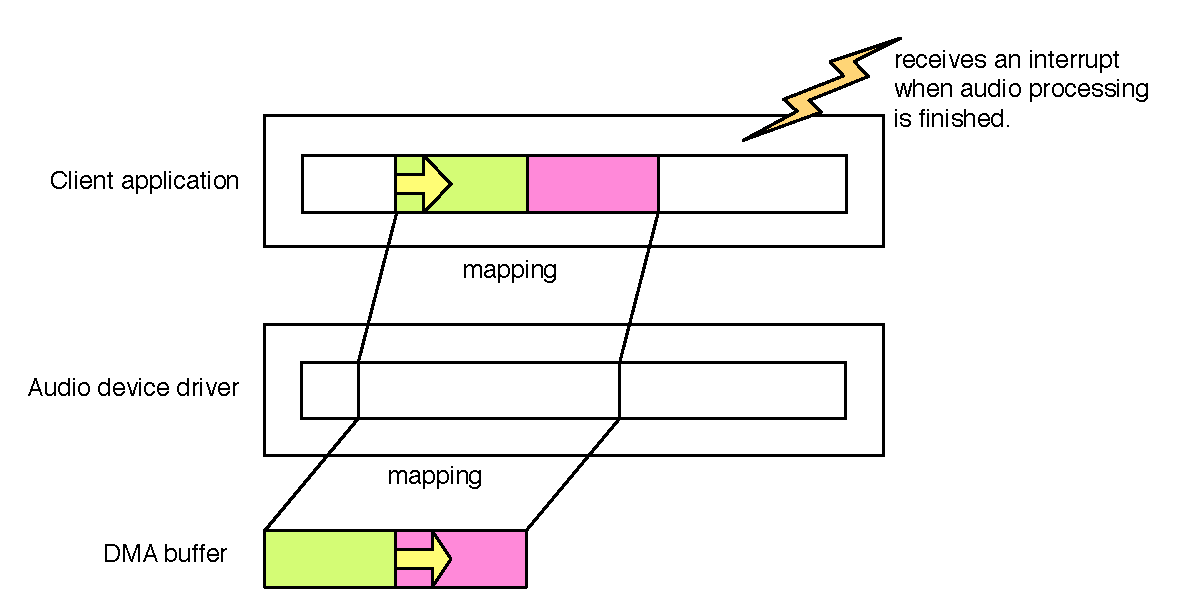
\includegraphics[scale=0.6]{audio_processing}
\caption{Audio playback mechanism}
\label{fig:audio_processing}
\end{center}
\end{figure}


\subsubsection{Recovery Handling \& Results}

Upon crash, the most important thing to ensure is that the audio playback in not interrupted, i.e. that the user perceives no gap in the audio playback while the driver recovers. This feature is easily supported by the DSP/DMA interaction and the fact that the application itself writes the audio data. DMA can be programmed such as it automatically restarts the same transfer again and again once it is finished. As the application directly writes audio data into the memory buffer transferred by the DMA to the card, this involves that once the card and DMA are programmed, audio playback continuity is handled by the application callback alone and do not rely on the audio driver being active.

Audio playback is therefore guaranteed as long as no system call is performed to stop the playback, change the card settings, or control the volume. Considering the frequency of these calls, and the speed at which the driver recovers, it is virtually impossible for the user or other applications to notice a crash and its successful recovery.

Some engineering still has to be performed on the driver to ensure successful recovery. The playback parameters must be kept for the eventuality the user wants to suspend and resume the playback.  This is because the playback parameters are only given when the playback is initialized. Also, for security reasons, the current owner of the audio device must be preserved to avoid interception by another process during the recovery. Finally, the DMA buffer mapping of the driver should also be preserved, as it is shared with the client application. All these features are easily obtained by making the relevant variables persistent.

The mixer settings are directly queried and setup to the sound card, and thus require no particular care across recovery because they do not reside in the driver's address space.

\subsubsection{Double-Buffered Variant}
We developed an alternative version of the audio driver that uses a double-buffering mechanism for the DMA buffer. Instead of directly mapping the DMA buffer to the client application, it maps another area of the driver's address space that the client application fills upon a sound card interrupt. The audio library then sends a message to the audio driver that copies the client buffer into the DMA buffer and acknowledge the end of interrupt to the hardware. This design can be justified by safety reasons (in the former design, the audio library, and therefore the client application, directly acknowledges the hardware, a situation that not all operating systems may allow) or to support other, older models of sound cards.

The only situation where the user would experience a gap in the audio playback would be when the user callback function has not finished committing its part of the audio buffer, but another interrupt is raised because the sound card finished playing the other half of the buffer. This situation can happen if the driver is too slow to recover. However, even in the case of a buffer size of 4096 bytes and audio settings of 44100Hz for 16 bits stereo playback, this would only happen if the driver takes more than 23ms to recover. As section \ref{sec:performance} shows, these delays should be respected on almost any machine.

\section{Discussion}
\label{s:discuss}

In this section, we discuss several further issues on the framework.

\subsection{Applicability to a Monolithic Kernel}

The framework is built on top of a microkernel which provides strong isolation of processes.  If one would like to port the framework to a monolithic kernel in which all system components are melted together, it is necessary to solve two isolation issues.

The first issue is fault containment.  A process on a microkernel is isolated from the kernel and other processes.  This guarantees fault containment; a failed process cannot make a wild write to another process or the kernel.  Under a monolithic kernel, isolation facilities like Nooks isolate a driver from the other parts of the kernel by means of the MMU isolation mechanism\cite{Swift2006}.  This means a driver runs as a process under Nooks and this approach introduces a large performance penalty because of the context switch cost implied by this design.  If another approach for fault containment, such as software fault isolation\cite{wahbe93efficient}, can be applied, the framework would work with a monolithic kernel with little loss of performance.

The second issue is isolation for communication.  Since a driver interacts with a user process through IPC, an IPC message is isolated from its local stack by the IPC mechanism, which means the driver is easily restarted without loosing the message from the user process.  On the other hand, a component in a monolithic kernel communicates via function calls.  Hence a message from the kernel is placed in a driver's local stack, which results in the message being lost on driver restart.  Thus, a special calling mechanism is necessary to preserve the message.  Again, Nooks provides a mechanism to switch the kernel stack to a dedicated stack when the execution path moves to a driver, and switch back it to the kernel stack when the call finishes.  The mechanism proposed in Nooks is therefore also applicable to our framework.

\subsection{Limitations}

There are several limitations to our approach.  First, a device driver in another operating system needs to be partially modified in order to work within ArcOS and the framework.  Introducing the restart handler and the persistent memory requires the driver to change its data structures.  More fundamentally, the libraries available in ArcOS may not be compatible with other operating systems. Some device drivers are probably required to undergo heavy modifications.  However, logic to manipulate a peripheral is common as long as the used hardware is the same.  Dissemination of IDL for device drivers such as Devil~\cite{merillon00devil} could improve the situation.

Second, recovery of drivers using shared memory areas is not fully supported.  Some device drivers use shared memory pages to share data with their clients so that they can transfer a large amount of data.  Those memory pages are directly mapped from the device driver's address space to the client's address space.  According to the L4 specification, if the device driver's address space is accidentally removed (by crash or whatever), the mapping path is changed such that the client is mapped from the source (in our case, P3 of the device driver).  After recovery of the device driver, it keeps the same memory page as before the crash from its P3.  Hence, the driver and the client can still have normal communications.  However, the mapping path is incorrect: if the client doesn't release the mapped pages when it terminates the communication with the device driver, it can still hold the memory pages that might be mapped to another client.  In the next release, we prohibit the direct memory mapping from a device driver to a client, and involve P3 so that such memory mapping is performed indirectly.

\section{Related Work}
\label{s:rel}

The existing device driver frameworks such as Windows Device Driver Kit\cite{wdm}, Apple's I/O Kit\cite{iokit}, and the one for Linux\cite{linuxdd} do not consider failure recovery in advance, even though device drivers have historically caused many problems.  We consider the reason why they do not support recovery features is to eliminate as much performance overhead as possible.  Indeed, device drivers under these frameworks run in kernel mode and are not isolated in order to reduce the interaction overhead between device drivers and the kernel.  However, considering the evolution of hardware, the overhead for improving the reliability of operating systems is acceptable.

Up to now, recovery of device drivers has been based on restarting. For instance, Nooks\cite{Swift2003}\cite{Swift2006} isolates device drivers from the rest of the kernel and is able to transparently restart them upon failure. A similar feature is provided by Minix 3 with the reincarnation server\cite{Herder2007}. These recovery mechanisms are all based on the assumption that the restarted driver has no state of its own.

This is unfortunately not the case of all device drivers as we discussed. For instance, character devices treat data as a stream and may fail in the middle of a transfer. In this case, simply restarting the driver and reissuing the faulty call may result in duplicated work being performed.  As opposed to these approaches, our approach is able to handle a driver with its internal state.

Another state that is important to preserve during recovery is the state of the managed hardware. Drivers typically initialize the hardware to an ``initial state'' and wait for instructions about how to control it. Such control put the hardware into a different state, and sudden reinitialization would cause a disruption in the user experience. Not to mention that applications calling the driver may still rely on the driver being in the pre-crash state, and may then issue commands that are not relevant to the reinitialized state, possibly causing the driver or the application itself to fail again.  Choices\cite{David2007} uses transactional memory to preserve the state of operations consistently.  However, they have no attempt to device driver recovery where the synchronization of software state and hardware state is necessary.

Another approach for making reliable device drivers is to write a device driver in a domain-specific language that is used for static analysis of device driver implementations\cite{merillon00devil}\cite{michael06solving}.  It checks how a device driver accesses a peripheral based on a description of the peripheral.  As discussed in the previous section, these domain-specific languages could reinforce our framework.

\section{Conclusion}
\label{s:sum}

This paper described a framework for developing resilient device drivers, which is efficient for failure recovery.  We aimed at developing a failure recovery mechanism only base on software technologies because of the limitations of embedded systems.

Choosing the microkernel architecture and providing a template of a device driver, our approach was able to build a light-weight failure recovery mechanism: small memory overhead and fast recovery.  Driver state is selectively stored in a persistent memory section, which, combined with a dedicated recovery entry point, allows the driver to easily preserve its important state across failures.  Since a driver developer is required to write a recovery procedure for each device driver, driver development is a little more observant.  Hence, we proposed a guideline to develop a device driver under our framework.  In addition, we showed the feasibility of the framework through a case study of three different classes of device drivers.


\bibliographystyle{unsrt}
\bibliography{references}

\end{document}

